% preamble

\documentclass[10pt]{article}
\usepackage[paperwidth=40in, paperheight=40in]{geometry}
\usepackage[usenames]{color} %used for font color
\usepackage{amssymb} %maths
\usepackage{amsmath} %maths
\usepackage{bm}
\usepackage[utf8]{inputenc} %useful to type directly diacritic characters

%%% Sans serif text font
\usepackage[scaled]{helvet}
\renewcommand*\familydefault{\sfdefault}\usepackage[T1]{fontenc}
%%%

\usepackage{skull}
\usepackage{tikz}
\usetikzlibrary{positioning}
\usetikzlibrary{arrows}
\usetikzlibrary{fit}
\usetikzlibrary{calc}
\usetikzlibrary{automata}
\usetikzlibrary{decorations.markings}
\usetikzlibrary{decorations.pathreplacing}

\tikzset{>=latex}
\tikzstyle{snode}=[black,draw=black,line width=1.5pt,shape=circle,fill=white,minimum size=8mm]
\tikzstyle{obnode}=[black,draw=black,line width=1.5pt,shape=circle,fill=black!20!white,minimum size=8mm]
\tikzstyle{detnode}=[black,draw=black,line width=1.5pt,densely dotted,shape=circle,fill=white,minimum size=8mm]
\tikzstyle{constnode}=[black,draw=black,line width=1.5pt,shape=rectangle,fill=white,minimum size=8mm]
\tikzstyle{mincnode}=[black,draw=black,line width=0.75pt,shape=rectangle,fill=white,minimum size=3mm]
\tikzstyle{blnode}=[white,draw=black,line width=1pt,shape=circle,fill=black,minimum size=1mm,font=\scriptsize,inner sep=1pt]
\tikzstyle{ylnode}=[black,draw=black,line width=1pt,shape=circle,fill=yellow,minimum size=1mm,font=\scriptsize,inner sep=1pt]
\tikzstyle{taro}=[->,line width=2pt,color=black]
\tikzstyle{thintaro}=[->,line width=0.75pt,color=black]
\tikzstyle{dtaro}=[->,line width=2pt, densely dotted,color=black]
\tikzstyle{smod}=[black, draw=black, line width=2pt, fill=white, shape=rectangle, rounded corners, minimum size=10mm, minimum width=20mm]
\tikzstyle{obmod}=[black, draw=black, line width=2pt, fill=black!20!white, shape=rectangle, rounded corners, minimum size=10mm, minimum width=20mm, minimum width=20mm]

\definecolor{shc}{RGB}{238,224,229}
\definecolor{shc2}{RGB}{182,152,195}
\definecolor{brnt}{RGB}{221,132,13}

\begin{document}
\begin{align*}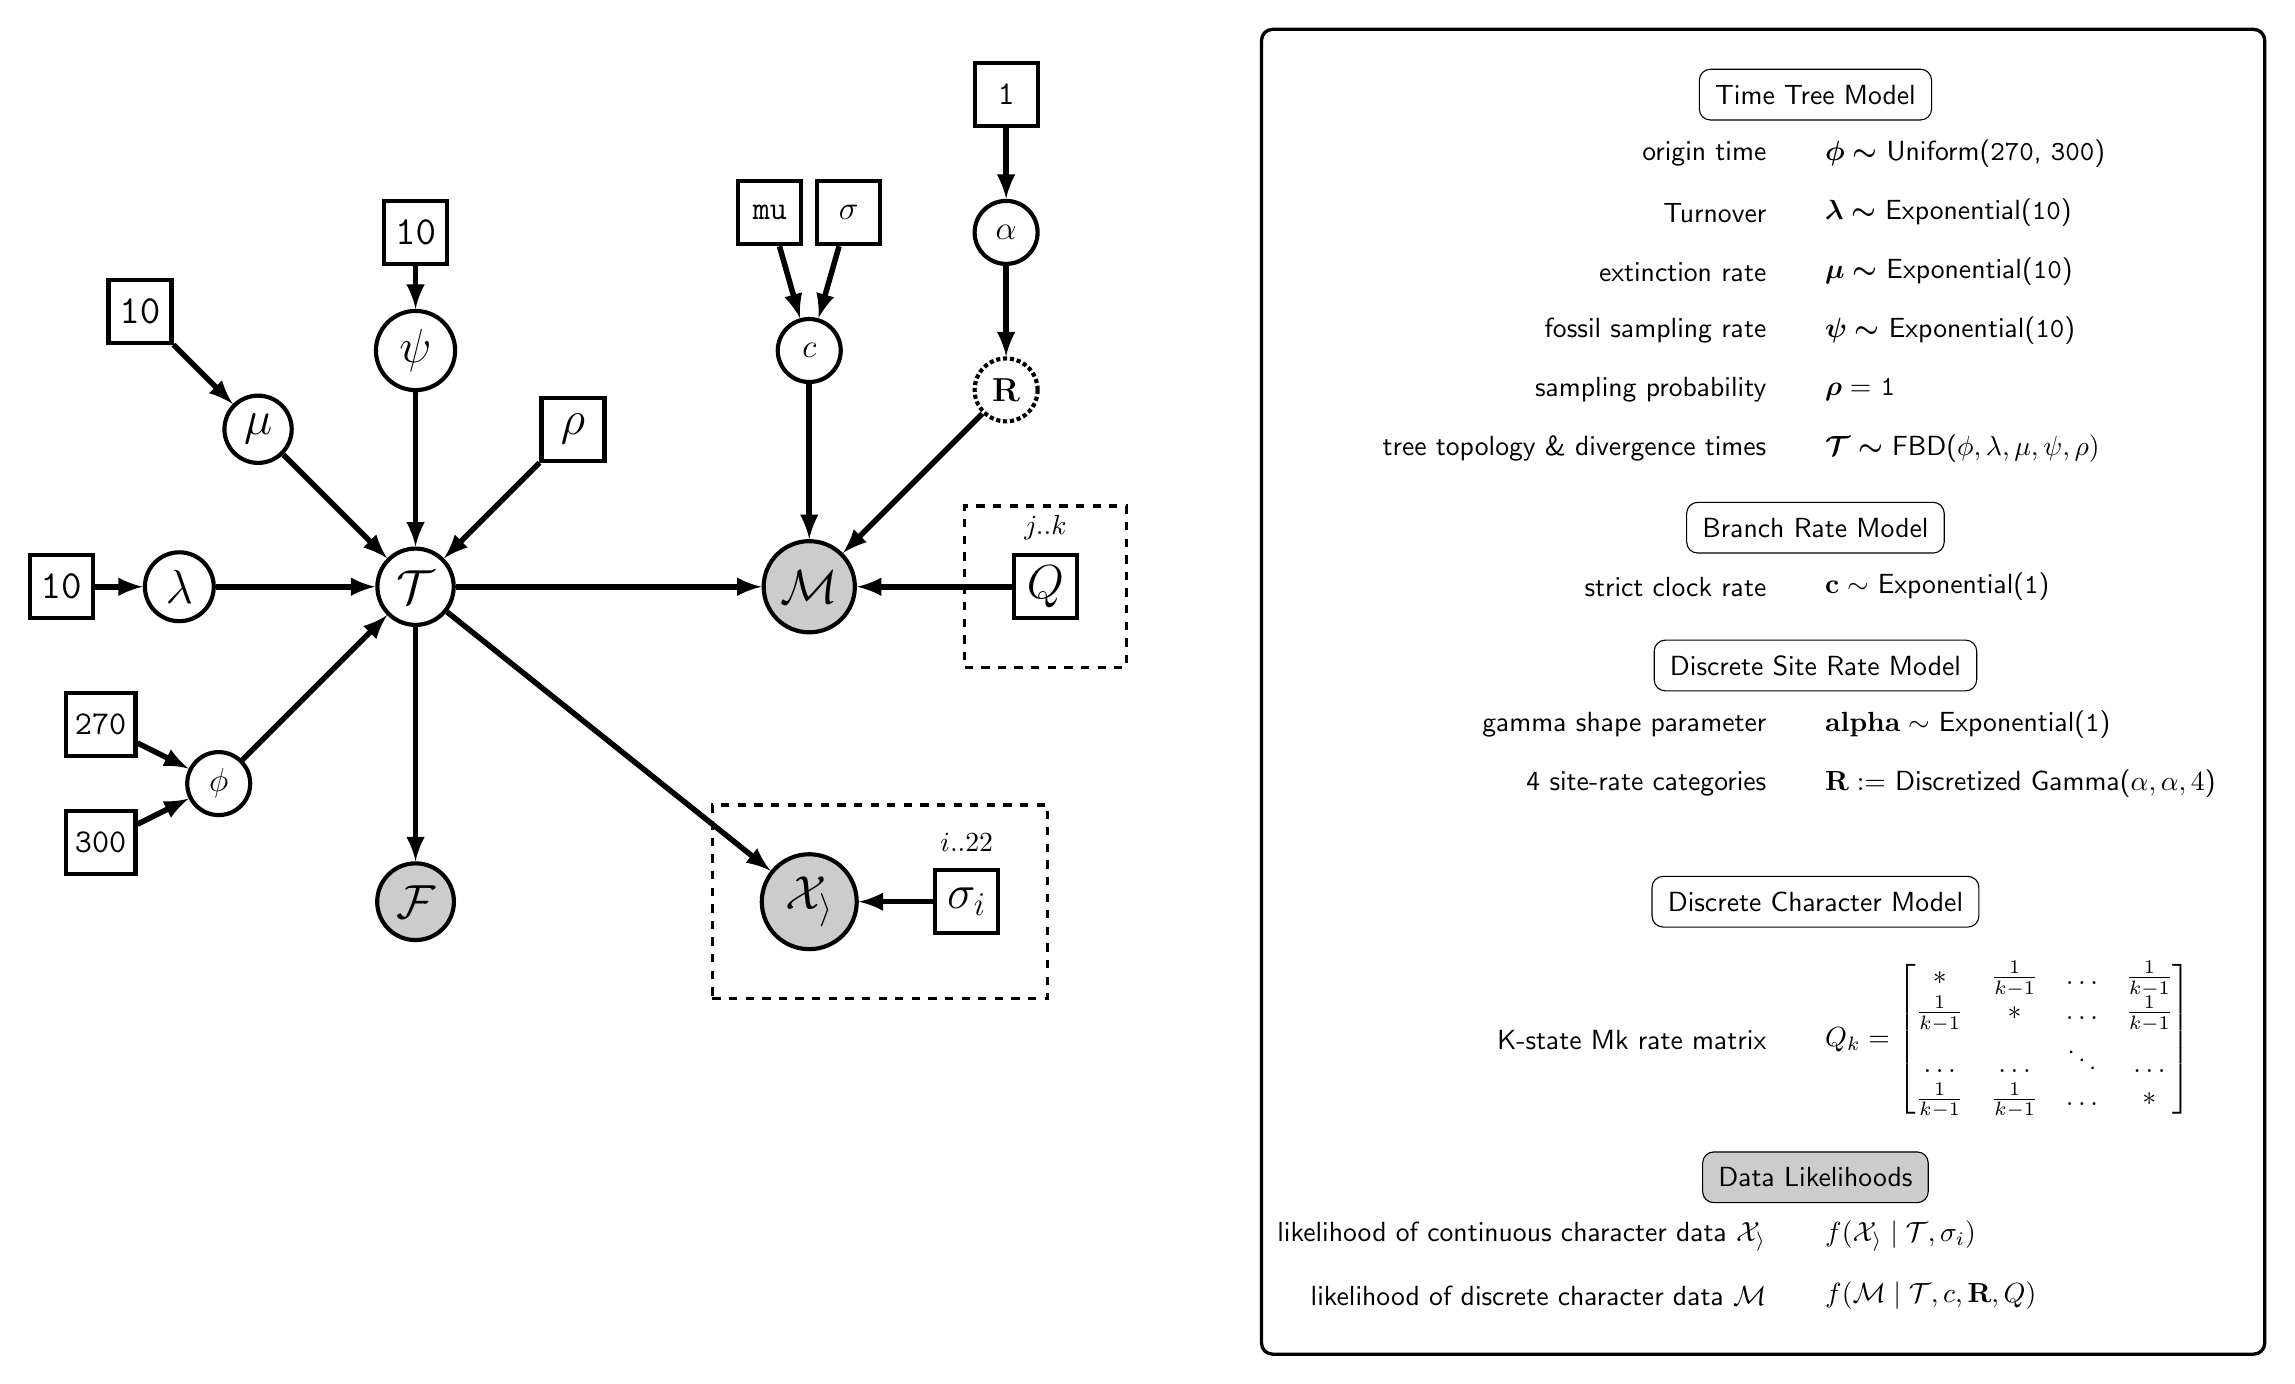
\begin{tikzpicture}
%\node (a1) at (-7.5,-7.75) {.};
%\node (a2) at (-0.5,-9) {.};
%\node (a3) at (-7.5,-9) {.};
%\node[rectangle, fill=shc3,inner sep=1mm, rounded corners, fit = (a1) (a2) (a3)] (siteplate) {};
%\node (la) at (-0.5,0) [left]{origin time};
%\node (ll) at (-0.5,-8.75) [left]{likelihood of morphological character data $\mathcal{M}$};
%\node[rectangle, fill=shc3,inner sep=3mm, rounded corners, fit = (la) (ll)] (siteplate) {};
%%%%% Time Tree Labels %%%%
\node[black, fill=white, draw=black, shape=rectangle, inner sep=2mm,rounded corners] (TTLabel) at (0,0.75) {Time Tree Model};
\node (origin) at (0,0) [right]{\bm{$\phi\sim$} Uniform({\tt 270}, {\tt 300})};
\node (la) at (-0.5,0) [left]{origin time};
\node (lambda) at (0,-0.75) [right]{\bm{$\lambda\sim$} Exponential({\tt 10})};
\node (lb) at (-0.5,-0.75) [left]{Turnover};
\node (mu) at (0,-1.5) [right]{\bm{$\mu\sim$} Exponential({\tt 10})};
\node (lc) at (-0.5,-1.5) [left]{extinction rate};
\node (psi) at (0,-2.25) [right]{\bm{$\psi\sim$} Exponential({\tt 10})};
\node (ld) at (-0.5,-2.25) [left]{fossil sampling rate};
\node (rho) at (0,-3) [right]{\bm{$\rho} =$ {\tt 1}};
\node (le) at (-0.5,-3) [left]{sampling probability};
\node (tree) at (0,-3.75) [right]{\bm{$\mathcal{T}\sim$} FBD($\phi, \lambda, \mu, \psi, \rho)$};
\node (lf) at (-0.5,-3.75) [left]{tree topology \& divergence times};
%%%%% Clock Labels %%%%
\node[black, fill=white, draw=black, shape=rectangle, inner sep=2mm,rounded corners] (ClkLab) at (0,-4.75) {Branch Rate Model};
\node (clock) at (0,-5.5) [right]{$\mathbf{c} \sim$ Exponential({\tt 1})};
\node (lg) at (-0.5,-5.5) [left]{strict clock rate};
%%%%% Site rate Labels %%%%
\node[black, fill=white, draw=black, shape=rectangle, inner sep=2mm,rounded corners] (SrLab) at (0,-6.5) {Discrete Site Rate Model};
\node (alph) at (0,-7.25) [right]{$\mathbf{alpha} \sim$ Exponential({\tt 1})};
\node (lh) at (-0.5,-7.25) [left]{gamma shape parameter};
\node (sr) at (0,-8) [right]{$\mathbf{R} :=$ Discretized Gamma($\alpha,\alpha, 4$)};
\node (li) at (-0.5,-8) [left]{4 site-rate categories};
%%%%% Subst rate Labels %%%%
\node[black, fill=white, draw=black, shape=rectangle, inner sep=2mm,rounded corners] (QmatLab) at (0,-9.5) {Discrete Character Model};
\node (qm) at (0,-11.25) [right]{$Q_k = \begin{bmatrix}
* & \frac{1}{k-1} & \ldots & \frac{1}{k-1} \\
        \frac{1}{k-1} & * & \ldots & \frac{1}{k-1} \\
        \hdots & \hdots & \ddots & \hdots \\
        \frac{1}{k-1} & \frac{1}{k-1} & \ldots & *
\end{bmatrix}$
};
\node (lj) at (-0.5,-11.25) [left]{K-state Mk rate matrix};
%%%%% likelihoods Labels %%%%
\node[black, fill=black!20, draw=black, shape=rectangle, inner sep=2mm,rounded corners] (likes) at (0,-13) {Data Likelihoods};
\node (foss) at (0,-13.75) [right]{$f(\mathcal{X_i}\mid \mathcal{T},\sigma_i)$};
\node (lk) at (-0.5,-13.75) [left]{likelihood of continuous character data $\mathcal{X_i}$};
\node (ddd) at (0,-14.5) [right]{$f(\mathcal{M} \mid \mathcal{T}, c, \mathbf{R}, Q)$};
\node (ll) at (-0.5,-14.5) [left]{likelihood of discrete character data $\mathcal{M}$};
%\node[rectangle, very thick, inner sep=3mm, draw=black!100, rounded corners, fit = (siteplate) (sr)] (boarder) {};
\node[rectangle, very thick, inner sep=5mm, draw=black, rounded corners, fit = (ll) (sr) (TTLabel)] (mm) {};
%%% GM %%%%
\node[snode] (tree) at ($(lg)+(-16,0)$) {\LARGE $\mathcal{T}$};
\node[snode] (lambda) at ($(tree)+(-3,0)$) {\LARGE $\lambda$};
\node[snode] (mu) at ($(tree)+(-2,2)$) {\LARGE $\mu$};
\node[snode] (psi) at ($(tree)+(0,3)$) {\LARGE $\psi$};
\node[constnode] (nul) at ($(lambda)+(-1.5,0)$) {\Large {\tt 10}};
\node[constnode] (num) at ($(mu)+(-1.5,1.5)$) {\Large {\tt 10}};
\node[constnode] (nup) at ($(psi)+(0,1.5)$) {\Large {\tt 10}};
%\node[white, fill=brnt, shape=rectangle, rounded corners] at ($(lambda)+(0,-1)$) {speciation rate};
%\node[white, fill=brnt, shape=rectangle, rounded corners] at ($(mu)+(0.6,0)$) [right]{extinction rate};
%\node[white, fill=brnt, shape=rectangle, rounded corners] at ($(psi)+(0,-1)$) [centered]{fossilization rate};
%\node at ($(lambda)+(0,0.75)$) {\scriptsize exponential};
%\node at ($(mu)+(0,0.75)$) {\scriptsize exponential};
%\node at ($(psi)+(0,0.75)$) {\scriptsize exponential};
\draw [taro] (lambda) -- (tree);
\draw [taro] (mu) -- (tree);
\draw [taro] (psi) -- (tree);
\draw [taro] (nul) -- (lambda);
\draw [taro] (num) -- (mu);
\draw [taro] (nup) -- (psi);
%\node at ($(nx)+(0,-1)$) {time tree};
%\node at ($(nx)+(0,-1.75)$) {Node ages};
\node[constnode] (rho) at ($(tree)+(2,2)$) {\LARGE $\rho$};
\draw[taro] (rho) -- (tree) ;
%\node[white, fill=brnt, shape=rectangle, rounded corners] at ($(rho)+(0,-1)$) {sampling probability};
\node[snode] (origin) at ($(tree)+(-2.5,-2.5)$) {\large $\phi$};
%\node at ($(origin)+(0,0.75)$) {\scriptsize uniform};
\draw[taro] (origin) -- (tree) ;
\node[constnode] (min) at ($(origin)+(-1.5,0.75)$) {\large {\tt 270}};
\node[constnode] (max) at ($(origin)+(-1.5,-0.75)$) {\large {\tt 300}};
\draw[taro] (min) -- (origin) ;
\draw[taro] (max) -- (origin) ;
%\node[white, fill=brnt, shape=rectangle, rounded corners] at ($(origin)+(0,-1)$) {origin time};
\node[obnode] (ddd) at ($(tree)+(5,0)$) {\LARGE $\mathcal{M}$};
\draw[taro] (tree) -- (ddd) ;
\node[obnode] (foss) at ($(tree)+(0,-4)$) {\LARGE $\mathcal{F}$};
\draw[taro] (tree) -- (foss) ;
\node[constnode] (qm) at ($(ddd)+(3,0)$) {\LARGE $Q$};
\node[rectangle,dashed, very thick, inner sep=6mm, draw=black!100, fit =(qm)] (siteplate) {};
\node at ($(siteplate)+(0,0.75)$) {$j..k$};
\draw[taro] (qm) -- (ddd) ;
\node[obnode] (ddc) at ($(tree)+(5,-4)$) {\LARGE $\mathcal{X_i}$};
\draw[taro] (tree) -- (ddc) ;
\node[constnode] (sigmaC) at ($(ddc)+(2,0)$) {\LARGE $\sigma_i$};
\draw[taro] (sigmaC) -- (ddc) ;
\node[rectangle,dashed, very thick, inner sep=6mm, draw=black!100, fit = (sigmaC)(ddc)] (siteplateC) {};
\node at ($(sigmaC)+(0,0.75)$) {$i..22$};
\node[snode] (clock) at ($(ddd)+(0,3)$) {\large $c$};
\node[constnode] (clockpar) at ($(clock)+(-0.5,1.75)$) {\large {\tt mu}};
\node[constnode] (clocksig) at ($(clock)+(0.5,1.75)$) {\large $\sigma$};
\draw[taro] (clock) -- (ddd) ;
\draw[taro] (clockpar) -- (clock) ;
\draw[taro] (clocksig) -- (clock) ;
\node[detnode] (sr) at ($(ddd)+(2.5,2.5)$) {\large $\mathbf{R}$};
\node[snode] (alph) at ($(sr)+(0,2)$) {\large $\alpha$};
\node[constnode] (alphpar) at ($(alph)+(0,1.75)$) {\large {\tt 1}};
%\node[rectangle,dashed, very thick, inner sep=7mm, draw=black!100, fit = (sr)] (siteplate) {};
%\node[anchor=south east,inner sep=7pt] at (siteplate.south east) {\small $i \in 4$};
\draw[taro] (sr) -- (ddd) ;
\draw[taro] (alph) -- (sr) ;
\draw[taro] (alphpar) -- (alph) ;
%\node[rectangle, very thick, inner sep=7mm, draw=shc2, rounded corners, fit = (foss) (rho) (nul) (nup)] (ttm) {};
%\node[anchor=north west,inner sep=7pt] at (ttm.north west) {\small Time Tree Model};
%\node[rectangle, very thick, inner sep=7mm, draw=shc2, rounded corners, fit = (ddd) (qm) (alphpar)] (mm) {};
%\node[anchor=north west,inner sep=7pt] at (mm.north west) {\small Morphological Data Model};
\end{tikzpicture}\end{align*}
\end{document}